\documentclass[12pt]{book}
\usepackage[T1]{fontenc}
\usepackage[utf8]{inputenc}
\usepackage[english]{babel}
\usepackage[cmex10]{amsmath}
\usepackage{amsfonts}
\usepackage{amssymb}
\usepackage{amsthm}
\usepackage{thm-restate}
\usepackage{gensymb}
\usepackage[linesnumbered,ruled,noend]{algorithm2e}
\usepackage[pdftex]{graphicx}
\usepackage{subfig}
\usepackage{mathtools}
\usepackage{tikz}
\usepackage{listings}
\usepackage{verbatim}
\usepackage{float}
\usepackage{hyperref}
\usepackage{cleveref}
\usepackage{setspace}
\usepackage{xpatch}

\graphicspath{{./images/}}
\DeclareGraphicsExtensions{.png}

\lstset{
  language=Python,
  basicstyle=\ttfamily\small,
  breaklines=false
}

\usetikzlibrary{positioning,chains,fit,shapes,calc}

\newtheorem{theorem}{Theorem}[chapter]
\newtheorem*{theorem*}{Theorem}

% not sure why cref now refers to algs as ``line''
\crefname{line}{algorithm}{algorithms}

\setcounter{tocdepth}{4}
\setcounter{secnumdepth}{4}


\DeclarePairedDelimiter{\ceil}{\lceil}{\rceil}
\DeclarePairedDelimiter{\floor}{\lfloor}{\rfloor}

\renewcommand{\vec}[1]{\ensuremath{\mathbf{#1}}}
\renewcommand{\l}{\left}
\renewcommand{\r}{\right}

\newcommand{\avec}[1]{\ensuremath{\tilde{\mathbf{#1}}}}
\newcommand{\ds}[1]{\ensuremath{\,\,#1\,\,}}
\newcommand{\dsand}{\ds{\land}}
\newcommand{\textds}[1]{\ds{\ds{\text{#1}}}}
\newcommand{\comma}{\ensuremath{\ds{\ds{\ds{,}}}}}
\newcommand{\toprove}{\ensuremath{\ds{\vdash}}}
\newcommand{\imply}{\ensuremath{\,\,\,\,\Rightarrow\,\,\,\,}}
\newcommand{\fromto}{\ensuremath{\rightarrow}}
\newcommand{\bigO}[1]{\ensuremath{\operatorname{O}\left(#1\right)}}
\newcommand{\bigW}[1]{\ensuremath{\operatorname{\Omega}\left(#1\right)}}
\newcommand{\bigT}[1]{\ensuremath{\operatorname{\Theta}\left(#1\right)}}
\newcommand{\R}[1]{\ensuremath{\,\mathbb{R}^{#1}\,}}
\newcommand{\trans}[1]{\ensuremath{\,{#1}^{T}\,}}
\newcommand{\func}[1]{\ensuremath{\operatorname{#1}}}
\newcommand{\inv}[1]{\ensuremath{{#1}^{-1}}}
\newcommand{\apos}[1]{\textsc{\char13}#1}
\newcommand{\prim}[1]{{#1}^\apos{}}
\newcommand{\ortc}[1]{\ensuremath{{#1}^{\bot}}}
\newcommand{\C}[1]{\ensuremath{\func{C}(#1)}}
\newcommand{\N}[1]{\ensuremath{\func{N}(#1)}}
\renewcommand{\dim}[1]{\ensuremath{\func{dim}(#1)}}
\newcommand{\abs}[1]{\ensuremath{\left\lvert #1 \right\vert}}
\newcommand{\norm}[1]{\ensuremath{\left\lVert #1 \right\rVert}}

\newcommand\xqed{%
  \leavevmode\unskip\penalty9999 \hbox{}\nobreak\hfill
  \quad\hbox{$\triangle$}}

\newcommand{\suchthat}{%
  \ensuremath{\mathrel{\,\,\ooalign{$\ni$\cr\kern-1pt$-$\kern-6.5pt$-$}}\,\,}}

\newcommand{\twopartdef}[4]
{
	\left\{
		\begin{array}{ll}
			#1 & \mbox{if } #2 \\
			#3 & \mbox{if } #4
		\end{array}
	\right.
}

\newcommand{\andspc}{\;\;\land\;\;}

\newcommand{\stcomp}[1]{\overline{#1}}

\newcommand{\apx}[1]{\widetilde{#1}}

\newcommand{\joinabove}[1]{\setlength\abovedisplayskip{0pt}}
\newcommand{\joinbelow}[1]{\setlength\belowdisplayskip{0pt}}

\newcommand{\Krylov}[3]{\mathcal{\func{K}}_{#3}(#1,#2)}

\hyphenation
{
a-ssign-ment
ori-gi-nal 
es-ta-bli-shes 
va-lues 
pre-ima-ges 
fo-llo-wing
cla-ri-fies
pro-per-ty
par-ti-cu-lar
mi-ni-mum
theo-rem
bet-ween
pro-per-ly
fac-to-ri-za-tion
si-mi-lar
auxi-lia-ry
ellip-soid
cons-truc-tive
pa-ra-lle-li-za-tion
pa-ra-lle-lism
pa-ra-llel
appli-ca-tion
either
com-ple-xi-ty
do-cu-ments
ho-mo-ge-neize
subs-trac-tion
po-ssi-ble
re-pre-sent
co-rrect-ness
easier
nu-me-ri-cal
des-cri-bed
LAPACK
BLAS
ins-ta-lled
mo-dern
cu-rren-tly
pro-ce-ssors
a-tten-tion
attrac-tive
aiming
eigenvalues
eigenvectors
se-cond
dis-connected
ge-ne-ra-ted
connec-ti-vi-ty
cons-traints
algo-rithms
massive
com-pa-ring
a-vai-la-ble
se-ria-lly
com-pu-ting
sca-la-ble
connected
}


\begin{document}
\begin{titlepage}
  \begin{center}
    \vspace*{1cm}

    {\Large \textbf{Symmetric Eigen Decomposition}}

    \vspace{0.5cm}
    A quest to find the fastest serial algorithm

    \vspace{1.5cm}

    \textbf{Darío Bahena Tapia}

    \vfill

    A thesis presented for the degree of\\
    Master in Computer Science

    \vspace{0.8cm}

    
\includegraphics[width=0.25\textwidth]{logo-cinves}

    \vspace{0.8cm}
    {
      \footnotesize
      Electrical Engineering Division, Computer Science Department\\
      Centro de Investigación y de Estudios Avanzados del Instituto Politécnico Nacional\\
      México\\
      2016
    }

  \end{center}
\end{titlepage}

\tableofcontents

\chapter{Definition of the Problem}

One of the main drivers for picking the thesis topic, was to enhance a
real life software product. The quest for such problem eventually
brought to the table a particular application which needs to calculate
an eigen decomposition of certain matrices; and which was finding such step
as a potencial bottleneck. To give a concrete example, a matrix of  $867
\times 867$ was taking 14 seconds on commodity hardware; and the
application needed to perform a serious of them in a row, which
potentially could accumulate to one minute. Those calculations are
to be done in the context of a single user request, for a implementing
a higher level functionality; thus, the time spent on the eigen
decomposition was a concern indeed. The concern raises mainly, with
the future expectation of handling much bigger matrices. \\

We adopted above problem as the thesis topic, and the purpose of this
chapter is to document the refinement of the
requirements we got, as well a some of the motivation and context of
the application (not too many, as we are talking about propietary
software whose details can not be disclosed). 

\section{Initial requirements}

The raw description of the problem was to speed up, as much as
possible, the eigen decomposition calculation described above. But
there were several restrictions or special requirements around such
calculation, which we list below:

\begin{itemize}
  \item The computation needs to be performed in the Java programming
    language, as the whole application is written in the same. \\
  \item The executing hardware is a commodity computer using Intel
    processors (exact definition of the machine used for testing
    appears on \cref{cha:exper}).
  \item We can not use multi-threading, the computation needs to occur
    serially (this relates to the application architecture, but we can
    not disclose more details about it). \\
  \item The matrix is symmetric (is equal to its transpose). \\
  \item All the eigenvalues are required, but only one eigenvector.
\end{itemize}
\hfill

The above list of requirements suggested that we needed to restrict
our attention to serial algorithms for the Symmetric Eigen
Decomposition (proper mathematical definitions will be provided on
\cref{cha:symm-eigen}). Such reduced scope was welcomed, as the whole
topic of Eigen Decomposition (usually called Eigenvalue Problem in
literature), is extensive enough to make its exploration prohibitive in
the few months we have to finish this project; specially because a big
part of the literature focuses on parallel/distributed algorithms, but
their serial versions could be still attractive for our purposes and
deserve attention. \\

However, the topic of Symmetric Eigenvalue Problem is still too wide. To give
the reader a sense of the topic's immensity, we want to mention that a
reestrictive search by title in Google Scholar
\cite{googlescholar}, brings almost 1000 references which contain the
words ``symmetric'' and ``eigenvalue''. Some of those references
are quite recent, which suggest is an active area of research. That is
not a surprise given the recent trends of BigData, Machine Learning
and Data Mining; which heavily rely on efficient Numeric Linear
Algebra algorithms. \\

The following sections detail a refinement of the initial
requirements, aiming to reduce the scope of our algorithm search. 

\section{The context of the calculations}

\subsection{Spectral Clustering}
Digging further into the application code, to which we got access
granted, allowed us to realize that the requirements were actually
more specific. The reason why all eigenvalues were required, was in
order to detect how many of them where zero; to be more specific,
whether we had more than one being zero \footnote{In real-life
  computer calculations, we do not really compare exactly against
  zero but with a quite small number; that represents a reasonable
  approximation to zero.}. These details
will not make much sense, unless we understand a bit more of the
application context. \\

The software application we are trying to optimize implements, among
many other things, some clustering
algorithms. The term Clustering might
ring a bell to the reader, as it is a trendy topic nowaways; specially
with algorithms like k-means (see for example \cite{rajaraman14}, a
quite pragmatic 
introduction to Data Mining at large scale, which devotes one chapter
to Clustering). The technique used by our the application is a bit
different though, to the classical approaches like k-means algorithm;
it uses something called Spectral Clustering, where information about the
eigenvalues and eigenvectors of an special matrix called the Laplacian
(built out of the domain data), are used to find the clusters within
the data. A gentle introduction to Spectral Clustering can be found in
\cite{luxburg07}. \\

\subsection{Algebraic Graph Theory}

Let us now talk a bit about an apparently disconnected topic: enter
Algebraic Graph Theory, which is a fascinating field that 
applies tools from Algebra to the understanding of graphs
(the canonical text books are \cite{biggs93} and \cite{godsil01}). The field
is rich enough to have subdivisions, and the one concerning us here is
the application of Linear Algebra machinery against matrices
associated to graphs; in particular the usage of eigenvalues or
eigenvectors of those matrices. Such branch is also called
Spectral Graph Theory, for which \cite{brouwer12} offers a compressed but
comprenhensive panoramic view. \\

Let $G = (V,E,W)$ be a weigthed undirected graph, where $V$ is the set
of vertices, $E$ is the set of edges and $W$ is an $n \times n$ matrix
with the positive weights associated to the edges ($n = |V|$). The
matrix used in Spectral Graph Theory that we care about is
called the Laplacian($L$), whose definition follows below: \\ 

\begin{align*}
  L_{ij} &= \twopartdef{\d_i}{i==j}{i \ne j}{-w_{ij}} \\\\
  \suchthat & d_i = \sum_{j=1}^n w_{ij}
\end{align*}
\hfill

A more compact definition of the Laplacian is $L = D - W$, where $D =
diag({d_1,d_2,\dots,d_n})$. There are actually two flavours of the
Laplacian, and the one defined here is referred as \emph{Unnormalized}
Laplacian in literature. \\

The Laplacian is a quite interesting matrix, in the sense that its
eigenvalues (also known as ``spectra''), reveal information about the
underlying graph G. In particular, about its connectivity. In this
regard, the theorem below will be cited later on the context of our
application: 

\begin{theorem}
  \label{thm:speconn}
  The algebraic multiplicity of zero as an eigenvalue of $L$ equals
  the number of connected components of $G$.
\end{theorem}
\hfill

Let us recall that the algebraic multiplicity \begin{footnote}For
  symmetric matrices like the Laplacian, the algebraic multiplicity
  equals the geometric multiplicity; where the later is defined as the
  dimension of the subspace generated by the eigenvectors associated
  with the eigenvalue. In that sense, for symmetric matrices there is
  no ambiguity and literature simply talks about the multiplicity of
  the eigenvalues. That happens in particular on the usual formulation
  of \cref{thm:speconn}.
  \end{footnote} of an eigenvalue, is the
number of times that it appears as a root of the characteristic
polynomial; while a connected component is a subgraph of
$G$ such that all its vertices are connected, but that as whole is not
connected with the rest of the graph. 
A condensed proof of this theorem is provided in
\cite{brouwer}, and a more detailed one appears in \cite{luxburg07}
(though not precisely in the context of Algebraic Graph Theory). \\

\subsection{The Connection between the two fields}

What does Spectral Clustering (performed by our application), have to
do with Algebraic Graph Theory? The former borrows its tools from the
second. As \cite{jia14} explains, the idea of Spectral Clustering is
to reduce the problem of data clustering to one of graph
partitioning. It does so by constructing an undirected graph with each
point in the dataset being represented as a vertex, and by defining a
similarity function 
between the points (vectors in \R{n} that represent our data items); such
function serves to build the weight matrix $W$ of the undirected weighted graph
$G = (V,E,W)$ we mentioned earlier. \begin{footnote}A typical choice
  for the similarity function is the Euclidian Distance, but there are
  other choices; see \cite{luxburg07} for further
  details.\end{footnote} Thus, we can perform partitions on the graph
based on certain cut methods, and call the resulting components as
clusters (whose vertices reference original points in \R{n}, that
compose our dataset). \\

It is on those cut methods, that the theorems of Algebraic
Graph Theory are used. The particular application we care about,
performs a bi-partition by employing the so called Fiedler Method; in
honor to Miroslav Fiedler, who wrote a seminal paper on both Algebraic
Graph Theory and Spectral Clustering, describing the actual
method. The idea is to calculate the eigenvector associated to the
second smallest value of the Laplacian matrix $L$ (called Fiedler
Vector), and use the sign of 
its elements to split the vertices of the graph in two
partitions. The technical details are in Fiedler's article
(\cite{fiedler73}), or in standard texts of Algebraic Graph Theory.
The intuitive idea is that the partitions generated by the Fiedler
Vector are ``good'', because they minimize the number of edges
required to split the graph; and to some extent the amount of edges
joining the two partitions tells us how close or distant are the
clusters that they represent in the original dataset. Actually,
Fiedler gave us an explicit metric for this connectivity of the graph;
it turns out that the eigenvalue associated with the Fiedler Vector
(second smallest eigenvalue), tells us how connected or disconnected
the graph is. Because of this, Fiedler baptized this eigenvalue as the
Algebraic Connectivity. \\

The following theorem is a corollary of \cref{thm:speconn}, 
it refers to the newly introduced concept of Algebraic Connectivity,
and serves as a further link between the two branches of Mathematics
that we briefly introduced: \\

\begin{theorem}
  \label{thm:algconn}
  The Algebraic Connectivity of $L$ is zero \iff $G$ is disconnected. 
\end{theorem}

This theorem is actually a corollary of \cref{thm:speconn}, for
the particular case of a connected graph. This is because the
Laplacian $L$ (a real, symmetric and positive semi-definite
matrix \footnote{A $n \times n$ positive semi-definite matrix $M$ is
  related to a 
  cuadratic form, and has the property of $\trans{\vec{x}}M\vec{x} > 0
\forall x \in \R{n}$, see \cite{strange88} for a review of this concept.}, exhibits additional properties: \\ 

\begin{itemize}
  \item All its eigenvalues are real and $ \ge 0$ (see \cite{strang88}). \\
  \item Zero is always its smallest eigenvalue (see \cite{luxburg07}).
\end{itemize}
\hfill

If we apply \cref{thm:speconn} to the case of a graph with a single
component (connected graph), then it would tell us that zero appears
once as an eigenvalue of its Laplacian ($L). Using the properties listed above, we
know that the second smallest eigenvalue (Algebraic Connectivity)
needs to be either zero or a 
positive number; but as we just stated that it can not be zero again, the
only other option is to be possitive. That could be translated into
proposition  ``A graph is connected $\iff$ it has an algebraic
connectivity $> 0$''; which can be reworded as follows if we negate both sides of
the logical equivalence: ``The
Algebraic Connectivity of a graph is zero $\iff$ it is
disconnected''. Latest rewording is essentially \cref{thm:algconn}.

\section{Final requirements}

The previous sections and the two theorems mentioned, were more than
just a cosmetic exercise; they have the practical purpose of
understanding better the current requirement, and also of proposing a
refinement that will help us to reduce the scope of our bibliographic
search. \\

On the context of Spectral Clustering, there is certain code in the
application that does a bi-partition of a graph. It does so by
calculating the Fiedler Vector, and splitting the nodes depending on
the sign of the vector elements. However, prior doing the
bi-partition, the application needs to verify if the graph is
connected (the Fiedler Vector will not help much if the graph has more
than one connected component). In order to detect the disconnected
case, the code leverages \cref{thm:speconn} and asks how many
eigenvalues of the Laplacian are 
zero. If there are more than one, then we have a disconnected graph
(which requires a different treatment); if there is just one, we
proceed to split the graph using Fiedler Vector. The pseudo-code of
this critical section would look like this: \\

\begin{algorithm}
  \label{alg:orig-code}
  \caption{Original calculation of the graph partition}
%
  \setstretch{1.35}
  \SetKwInOut{Input}{Input}
  \SetKwInOut{Output}{Output}
  \DontPrintSemicolon
%
    \Input{Laplacian matrix $L$ of the graph}
%
    \Output{A partitioned graph $G$}
%
    $evals, evecs = \func{calculate-all-eigenvalues-and-eigenvectors}(L)$ \;
%    
    \If {$|e \suchthat ev \in evals \and ev ~ 0| > 1$}
    {
      \text{disconnected case, special treatment for $G$ using both $evals$ and $evecs$} \;
    }
    \Else
    {
      \text{connected case, regular bi-partition of $G$ using Fiedler Vector (already calculated)} \;
    }
\end{algorithm}
\hfill

Under the assumption that the connected case is more common than the
disconnected one, we can propose the first high level
optimization. Theorem \cref{thm:algconn} tells us that, in order to
detect the disconnected case, we do not need  to calculate all the
eigenvalues of $L$; the Algebraic Connectivity (second smallest) is
enough. Thus, the proposed new logic can go like this: \\

\begin{algorithm}
  \label{alg:optim-code}
  \caption{Proposed calculation of the graph partition}
%
  \setstretch{1.35}
  \SetKwInOut{Input}{Input}
  \SetKwInOut{Output}{Output}
  \DontPrintSemicolon
%
    \Input{Laplacian matrix $L$ of the graph}
%
    \Output{A partitioned graph $G$}
%
    $ac, fv = \func{calculate-algebraic-connectivity-and-fiedler-vector}(L)$ \;
%    
    \If {$ac ~ 0$}
    {
       $evals, evecs = \func{calculate-all-eigenvalues-and-eigenvectors}(L)$ \;      
      \text{disconnected case, special treatment for $G$ using both $evals$ and $evecs$} \;
    }
    \Else
    {
      \text{connected case, regular bi-partition of $G$ using Fiedler
        Vector $fv$} \;
    }
\end{algorithm}
\hfill

For the cases of disconnected graphs, we would need to
calculate twice the Algebraic Connectivity and Fiedler Vector; but
those are expected to be rare cases. \\

With the proposed change we are opening the door for leveraging the
properties of the Laplacian matrix $L$, which symmetric, sparse and
positive semi-definite. While we have mentioned what it means to be
symmetric ($L = \trans{L}$) and positive semi-definite ($\forall x \in
\R{n} \trans{\vec{x}}L\vec{x} > 0$); the sparsity deserves a few
words. Intuitively, an sparse matrix has ``mostly zeros'', though that
is a quite open definition subject to arbitrary interpretations; how many
are ``mostly''? According to \cite{richard12}, in practice a matrix
with more than $50$\% of zero entries can be considered sparse. The
sample $867 \times 867$ matrix we mentioned on the first section,
which is expected to be a representative input, falls into this
definition; it has around $70$\% of (nearly) zero entries. This
sparse characteristic of the Laplacian is quite relevant for our
investigation, as the numeric algorithms for solving the Symmetric
Eigenvalue Problem are clearly divided in two big branches: those
attacking the non sparse (dense) matrices, and those covering the
sparse ones. \\

Furthermore, the algorithms specialized for sparse matrices tend to
focus on calculating just a few eigenvalues/eigenvectors; that fits
perfectly well on the proposed logic, which just requires a single
pair. This does not necessarily mean that we are totally discarding
the dense matrix branch of algorithms. For the rare but still possible
case of a disconnected graph, we want to use something better than
offering of the Colt library; as it uses the classical
algorithm known as \emph{QL} (see \cref{sec:trid-ql}); based on routine
\emph{TQL2} of the
70's Fortran77 library EISPACK (\cite{eispack}). Such library has been
superseded by LAPACK (\cite{lapack}); and in particular, the
equivalent of routine \emph{TQL2} has been improved (see
\cref{sec:mr3}). As the sparse routines are designed for calculating a
few eigenvalues/eigenvectors, it would make sense to continue using a
dense matrix algorithm for the disconnected case, but leveraging
modern LAPACK implementations (see \cref{cha:lapack}). \\

Going further, there are algorithms specifically tailored for
calculating the Fiedler Vector and its associated eigenvalue
(Algebraic Connectivity). We also want to include those in the
comparison (see \cref{cha:trmin-fiedler}). \\

A final consideration is that, while the serial nature of the
algorithm remains as a requirement (no parallelism), there is no
restriction for recommending the usage of vectorized kernels like BLAS
(\cite{blas}); which is actually used by LAPACK and other higher level
libraries. BLAS (Basic Linear Algebra Subroutines), is a mature
industry standard, that hardware vendors implement for their
processors; in particular Intel leverages its vector facilities SSE
(Intel seems to be the commodity processor that the application can
rely on). \\

Taking into account the new understanding of the problem, we proceed
to list the refined requirements: \\

\begin{itemize}
  \item Goal is to reduce the time spent solving the Symmetric Eigenvalue
    Problem. \\
  \item The matrix against which we compute the eigenvalues and
    eigenvectors is the Laplacian of a graph; expectation is to seek
    for algorithms that leverage its qualities (symmetric, sparse and
    positive semi-definite). \\
  \item The computation needs to be performed in the Java programming
    language, as the whole application is written in the same. \\
  \item The executing hardware is a commodity computer using Intel
    processors (exact definition of the machine used for testing
    appears on \cref{cha:exper}).
  \item We can not use multi-threading, the computation needs to occur
    serially. There is no restriction
    though, in suggesting the usage of vectorized routines for Intel
    processors; like those present in BLAS library. \\
  \item Assuming that the disconnected graph case is uncommon, we
    still want to calculate there all eigenvalues and eigenvectors;
    but with a newer algorithm for dense matrices (like those present
    in LAPACK library). \\
  \item For the common case of a connected graph, we shall calculate
    only the algebraic connectivity and its associated Fiedler
    Vector (see psedo-code from  \cref{alg:optim-code}).
\end{itemize}
\hfill

\section{Expectation and outline of the thesis}
Being this a master degree thesis, is not expected nor feasible due
time constraints, that we come up with a new algorithm (that would be
suitable for a PhD thesis). Then, expectation was to search what are
the available algorithms; and to evaluate their performance under the
cited requirements. Detailed descriptions of the algorithms is
expected though, along with proper explanation of why some performed
better than others. Ultimate expectationis that, with the suggested
optimization, the application becomes able to cover new use-cases
involving bigger data sets (bigger Laplacian matrices). \\

The outline of the rest of this thesis is as follows: \\

\begin{itemize}
  \item \cref{symm-eigen} gives an introduction to the generic problem
    we want to solve faster, The Symmetric Eigenvalue Problem. We also
    include here, a brief overview of the numerical aspects that need
    to be considered when evaluating the algorithms (numerical
    stability and ill-conditioned data). \\
  \item \cref{lapack} covers three dense-matrix algorithms that come bundled with
    LAPACK, the first one is the QR algorithm; which is not really one
    of the proposed candidates, but rather the theoretical background
    of the Colt implementation. This chapter also includes the first two
    candidates for the experiment phase: the MR3 and the
    Divide-and-Conquer algorithms; both included as well in LAPACK. \\
  \item \cref{ir-lanczos} covers the first sparse-matrix algorithm to
    evaluate, the Implicitly Restarted Lanczos (available in a Java
    port of ARPACK \cite{arpack}). \\
  \item \cref{lobpcg} introduces the second sparse-matrix proposal,
    the Locally Optimal Block Preconditioned Conjugate Gradient
    Algorithm (LOBPCG). This is perhaps the most modern algorithm, and
    the only one incorporating preconditioning of the data. The Java
    implementation is available thanks to Sparse Eigensolvers for Java
    Project (\cref{sparseigensolvjava}).\\
  \item \cref{trmin-fiedler} explains the most specialized candidate
    of the proposal, the TraceMin-Fielder Algorithm; which was designed
    specifically for calculating only the algebraic connectivity and
    the Fiedler Vector. The expectation is that this algorithm beats the rest
    during the experiments, as is the one taking into account more
    properties of the matrix $L$ (see \cref{cha:exper} to find out if
    this expectation matched reality). There is no Java implementation
    available, but we will port the Python version found in Networkx
    Project \cite{networkx}. 
  \item \cref{exper} describes the experimentation phase, including
    the details of the commodity hardware, as well as the matrices
    used for comparing the different algorithm
    implementations (we included the provided $867 \times 867$
    matrix, but also other ones from standard benchmarks
    available). The performance observed (memory and cpu) are reported
    on this chapter, across the different combinations of algorithms
    and matrices. \\
  \item \cref{conclu} The conclusions chapter interprets the results,
    explaining why certain algorihtms performed better than others,
    under the experiment setting. It includes the final recommendation
    for the application stakeholders.
\end{itemize}


\chapter{The Symmetric Eigenvalue Problem}
\label{cha:symm-eigen}

\chapter{LAPACK Algorithms for Dense Matrices}
\label{cha:lapack}
\section{The Implicit QL Algorithm}
\label{sec:trid-ql}

\section{MRRR Algorithm}
\label{sec:mr3}

\section{Divide and Conquer Algorithm}
\label{sec:div-conq}


\chapter{Implicitly Restarted Lanczos Algorithm}
\label{cha:ir-lanczos}

 \begin{frame}
  \frametitle{LOBPCG}
  \begin{block}{Ancestor (dense eigensolver $2 \times 2$)}
    Preconditioned Steepest Descent Algorithm applies Rayleigh-Ritz
    against $\func{span} \{\vec{x}_i, T\vec{r}_i\}$
    ($T$ is a preconditioner) $\suchthat$
    \[
    \joinabove{0}
    \vec{r}_i = A\vec{x}_i - \func{\rho}(\vec{x}_i)\vec{x}_i
    \ds{\land}
    \func{\rho}(\vec{x}) = \dfrac{\trans{\vec{x}}A\vec{x}}{\trans{\vec{x}}\vec{x}}
    \joinbelow{0}
    \]
  \end{block}
  \begin{block}{Main ideas (dense eigensolver $3 \times 3$)}
    Uses subspace $\func{span} \{\vec{x}_i, T\vec{r}_i, \vec{x}_{i-1}\}$ to
    accelerate convergence (in practice $x_{i} - \beta x_{i-1}$); Knyazev also
    proved that $T$ must be SPD to guarantee convergence. His algorithm also features constraints $Y$ (search in $\ortc{Y}$).
  \end{block}
  \begin{block}{Practical considerations (NetworkX)}
    \begin{itemize}
    \item We set $k=1$ and $Y = \vec{1}$.
    \item $T = \dfrac{1}{\func{diag}(A)}$ (SPD)
    \item Numerical errors on clustered eigenvalues.
    \end{itemize}
  \end{block}
\end{frame}

%%  LocalWords:  Antecessor

\chapter{TraceMin-Fiedler Algorithm}
\label{cha:trmin-fiedler}

\chapter{The Experiment}
\label{cha:exper}

\section{Setup}

\subsection{Hardware}

All the tests were conducted on a laptop with a commodity processor
(Intel\textregistered Core\texttrademark $\,i5$ at $2.40$GHz). In
order to enforce serial execution, even
when low level libraries attempted multi-threading \footnote{We are talking about BLAS 
  or LAPACK; as the high level algorithms used were serial.}, we used
the Linux  
\emph{taskset} command. The laptop has $8$Gb of RAM, but no more than 512Mb
were used on each experiment (and only for dense matrix algorithms;
sparse ones used much less). \\

\subsection{Software}

The implementations of the algorithms we used, were basically Python
wrappers against native libraries. These packages were SciPy
\cite{scipy} and NetworkX \cite{networkx}. On the other hand, the
native libraries actually offering the algorithm implementations were:

\begin{itemize}
  \item LAPACK \cite{lapack}, which provides (among many other things)
    the \gls{MRRR} implementation. LAPACK is actually the industrial
    standard for dense matrix computations. LAPACK is implemented in
    Fortran90 \footnote{At least the opensource version we used, as
      there are other commercial implementations as well.}.

  \item ARPACK \cite{arpack}, which provides the variant of the
    Lanczos algorithm that we tested (IRLM). It also relies on LAPACK
    as a lower layer. ARPACK is implemented in Fortran77.

  \item Scipy \cite{scipy}, which delivers the implementation of
    LOBPCG that we tested. While Scipy may also use LAPACK for several
    operations, is interesting that LOBPCG is the only algorithm that
    is implemented in Python. This makes reading its code a much
    easier task, than say, reading it from the Fortran77 ARPACK. 
\end{itemize}

As it can be perceived, all the algorithm implementations ultimately
rely on LAPACK; and this in turn, relies on BLAS \cite{blas}. All
those libraries were installed on the laptop, of course. Finally, the
\gls{SCC} algorithm is offered by the Scipy package as well 
(\emph{scipy.sparse.csgraph.connected\_component}). Last but not least, same SciPy also provides the sparse formats tested (CSR and CSC). \\

Overall, Scipy makes quite accessible a lot of scientific
software; it feels like a new generation MATLAB that is becoming more
and more popular \footnote{A new competitor entered the arena
  recently, namely the Julia Programming language; specifically
  designed for scientific computing. We tried this language as well,
  for some of the experiments; but ended up preferring the maturity
  and wider repertoire of the Python + SciPy combo.}. Another merit of Scipy,
is that its performance is quite close to that of native code (we
also tested calling the libraries, like ARPACK, from low level C
code). The little penalty in performance by using the Python wrappers,
is definitely worth it in terms of development productivity. 

\section{Data Preparation}

\subsection{The actual data}
We created 10 random matrices from application's domain data, using
the same encoding techniques they use in production. The sizes of such
matrices are in the range $[867,4500]$, so they fit in memory without
problem. \\

\subsection{Sparse formats}
Two sparse matrix formats were tested with Lanczos and LOBPCG
algorithms; namely the Compressed Sparse Row (CSR) and Compressed
Sparse Column (CSC) formats. For an overview of these and related
formats, in the actual context where we experimented with them, the
reader can consult \cite{johansson15}. While both formats showed
similar performance results, we prefer CSR because is the preferred
format to use with the \gls{ClusteredEigenvalues} removal pre-processing (see
below). 

\subsection{Avoiding \gls{ClusteredEigenvalues}}
\label{sub:avoid-clust-eigv}

As we mentioned on previous chapter, \gls{ClusteredEigenvalues} were a
headache for both Lanczos and LOBPCG; so we needed to do something
about them. By researching deeper why they were occurring, we found
that for the graphs behind the \gls{Laplacian}s produced by the
application, there was a common pattern: a disconnected graph with a
2-3 node small component, and the rest of the nodes in another big
component. \\

The theory says that for a disconnected graph of two components, the
first and second eigenvalues of the \gls{Laplacian} will be zero (see
\cite{luxburg07}). In practice, what you get instead are two very
small numbers; and that is an extreme case of clustered
eigenvalues. They are very close to each other, because both try to
approximate zero. \\

The solution for this issue was to simply remove the already
disconnected small component; it makes sense given that ultimately,
the high level operation we want to perform on the graph is a
bi-partition (thus, expectation is that the graph is connected). The
caveat was to compute the Strongly Connected Components (\gls{SCC}) and the
new weights matrix quite efficiently, such that this pre-processing
did not become a performance penalty. The \gls{SCC} computation can be done
efficiently (sub-second) with algorithm documented in \cite{pearce05},
for which we did not dig its internals but just used the
implementation available in SciPy. This  
algorithm/implementation actually, is the reason why we prefer CSR
format over CSC (if the weights matrix is not passed in CSR format,
the routine takes much more time). \\

The re-computation of the weights matrix $W$ though, required bit more
of thought. It turned out that the CSR format is not very friendly
with row/column removal operations (which we need to do, in order to
simulate that nodes got removed from the graph). Based on an
StackOverflow post \cite{alim15}, we took the idea of using an
intermediate sparse sparse format (COO) which allows for faster
column/row removals; but at the same time, it also allows for fast CSR
conversion. The current StackOverflow post has an even faster option
published now, but the Python code below was good enough for our
experiments (it showed an overall time of $1.2$ secs for the biggest
matrices). \\

    \begin{lstlisting}
def split_cc_sparse2(W, cclab):
    idx_del = np.nonzero(cclab)[0]
    keep_row = np.logical_not(np.in1d(W.row, idx_del))
    keep_col = np.logical_not(np.in1d(W.col, idx_del))
    keep = np.logical_and(keep_row, keep_col)
    W.data = W.data[keep]
    W.row = W.row[keep]
    W.col = W.col[keep]
    W.row -= np.less.outer(idx_del, W.row).sum(0)
    W.col -= np.less.outer(idx_del, W.col).sum(0)
    k = len(idx_del)
    W._shape = (W.shape[0] - k, W.shape[1] - k)
    return W
    \end{lstlisting}
    \joinbelow{1cm}
    
The snippet above works as follows: the argument
\emph{cclab} contains the node labels for the components, namely $0$ and $1$
for the big and small ones respectively. Our goal is to eliminate the nodes with
label $1$ from the weights matrix $W$. For that, that lines $2-8$
begin by shrinking the index and data arrays (after removal of unwanted
columns/rows); then lines $9-10$ eliminate the potential gaps on the
indices and finally lines $11-12$ truncate the $W$ matrix to the new
size. The key idea is to do all the operations in terms of the NumPy
array primitives, which are quite efficient. 

\subsection{Shifting the spectra}

The \gls{Cholmod} linear solver mentioned on the previous chapter, requires
that the matrix is Symmetric Positive Definite; and the \gls{Laplacian} is
not (it is symmetric, but has
one zero eigenvalue). Doing a little shift on the eigenvalues ($L +
0.01I$), makes the \gls{Laplacian} Positive-Definite as required; and at the
end of the algorithm execution, we can just subtract the same shift to
the obtained eigenvalue to get the actual answer (which is not really
that relevant, as we mostly want the eigenvector; the eigenvalues are
just side products that the algorithms also produce). 

\section{Results}

Though the laptop was idle at the time of the experiments, we captured
execution times as averages out of 100 executions (for each
algorithm/matrix combination). The graph below shows the results
obtained by encoding the matrices in CSR format. We present a
two-dimensional graph, with the X-axis representing the matrix size
and the Y-axis the average execution time in seconds. 

\begin{figure}[H]
  \centering
  \caption{Experiment Results in CSR format}  
  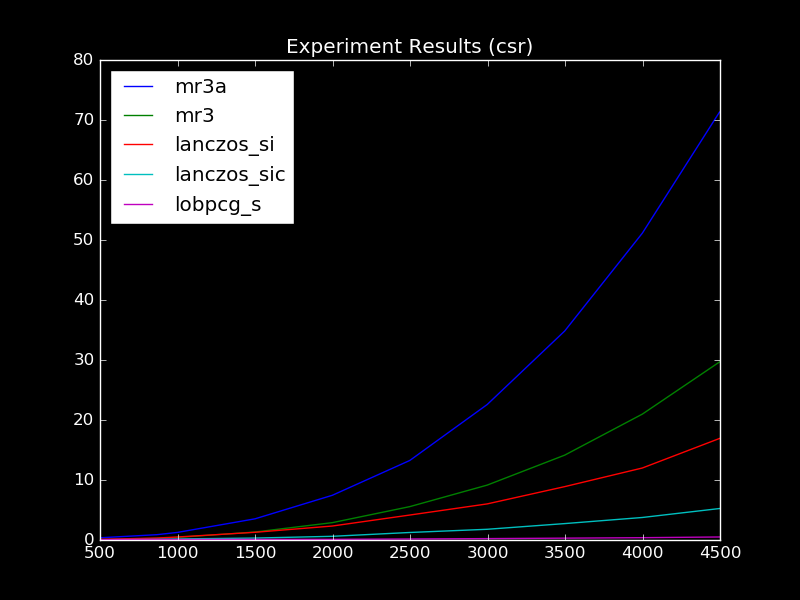
\includegraphics[width=11cm,height=8cm]{results-csr}
\end{figure}

Let us review each line in more detail (we talk mainly about the times
for the biggest matrix):

\begin{itemize}
\item The green line (label \emph{mr3a}) represents the times for the
  \gls{MRRR} algorithm, for 
  computing all the eigenpairs. This is not exactly the same time
  the application will get today, as the algorithm is different; but
  it could be considered as a lower bound (given that \gls{MRRR} is the
  state of the art for dense matrices). We can see that the time for
  the biggest matrix goes a bit higher than 70 seconds.
\item The blue line (label \emph{mr3}) is also the \gls{MRRR} algorithm, but
  taking advantage of its main feature: the ability to compute in
  isolation just the eigenpair we need. We can see that doing so,
  reduces the time to a bit less than 30 seconds (for the biggest
  matrix).
\item The orange line (label \emph{lanczos\_si}) is the first sparse
  matrix algorithm; it consists in the Lanczos variant using \gls{SuperLU}
  as the linear solver. Even when such solver is not specialized for
  the \gls{Laplacian} matrix, it can reduce the time to a bit less than 20
  seconds.
  \item The sky blue line (label \emph{lanczos\_sic}) is the very same
    Lanczos variant, but this time using the \gls{Cholmod} linear solver. We
    can see that using a more specialized solver, that is optimized
    for Symmetric Positive Definite matrices, pays off; to biggest
    time does down to 5 seconds, approximately.
  \item The Lanczos variant (\gls{IRLM}), combined with \gls{Cholmod} linear
    solver, was going to be our best time; until we discovered how to
    avoid the exceptions that the \gls{LOBPCG} implementation was raising on
    the presence of \gls{ClusteredEigenvalues}. That brought this purple
    line (label \emph{lobpcg\_s}), which by far beats them all; the time
    goes into sub-second scale even for the biggest matrix (the actual
    average time is around half a second, sometimes a bit bigger but
    still within a second). This makes \gls{LOBPCG} the definite winner of
    the experiment. 
\end{itemize}

Even with an apparent idle laptop,
  and with \emph{taskset} command, there were still variations on the
  average times; a more precise mechanism could be to boot the laptop
  into an special mode where there are less admin tasks running on the
background. This was not considered critical for our experiment, as
the pattern in the execution times was consistent; only difference was
a shift of the whole pattern (but \gls{LOBPCG} times remained in sub-second
scale). \\ 

Putting aside the fluctuations mentioned above; the CSC results are
basically the same than the CSR ones. A sample execution is shown
below: 

\begin{figure}[H]
  \centering
  \caption{Experiment Results in CSC format}   
  \includegraphics[width=11cm,height=8cm]{results-csc}
\end{figure}

Even when both formats behave well with the sparse algorithms, we
prefer CSR for reasons explained already on this chapter.

\section{Why \gls{LOBPCG} beats \gls{IRLM}?}
\label{sec:why-lobpcg}

The dramatic advantage that \gls{LOBPCG} shows against
Lanczos/\gls{IRLM} calls for our attention, and for an attempt to
explain why it occurred; we will do so based on the theory presented
in \cref{cha:algs}. The \cref{tab:lanczos-vs-lobpcg} summarizes all
the advangates 
that we see in \gls{LOBPCG} over Lanczos/\gls{IRLM}; and the rest of
this section will detail each point.

\begin{table}[h]  
  \caption{Lanczos vs LOBPCG}\label{tab:lanczos-vs-lobpcg}
  \begin{tabular}{l | c | c | }
    Feature/Issue & Lanczos(IRLM) & LOBPCG (single) \\
    \hline \hline
    Need Restarting &
    Yes, due $\Krylov{\inv{L}}{\vec{x}_0}{m}$ &
    No, $\func{span} \{\vec{x}_i, T\vec{r}_i, \vec{x}_{i-1}\}$ \\
    \hline
    Search strategy &
    Plain search &
    $\nabla (\func{\rho}(\vec{x_i}))$ \\
    &
    &
    $\suchthat \vec{r}_i = L\vec{x}_i - \func{\rho}(\vec{x}_i)\vec{x}_i$\\
    \hline
    Search Constraints &
    No &
    Yes ($\ortc{Y} = \ortc{\vec{1}}$) \\
    \hline
    Requested spectra &
    $k=2$ &
    $k=1$ \\      
    \hline
    Matrix operation &
    solve $L\vec{x} = \vec{b}$ &
    $L\vec{x}$ \\
    \hline      
    Uses Preconditioning &
    Only with iter solvers &
    Yes $\left(T = \dfrac{1}{\func{diag}(L)} \right)$ \\
    \hline
    Clustered eigenvalues &
    Inherited from PM &
    Bug? \\      
    \hline
  \end{tabular}
\end{table}

\subsection{No need for restarting}

Given that \gls{LOBPCG} uses a fix-size generator set for the
search-subspace, $\func{span} \{\vec{x}_i, T\vec{r}_i,
\vec{x}_{i-1}\}$, it does not need to invest extra time ensuring the
size remains low; contrary to \gls{IRLM}, which needs to
ensure the dimension of $\Krylov{\inv{L}}{\vec{x}_0}{m}$ does not grow
too much (causing unbounded memory consumption).

\subsection{Clever search strategy}

While \gls{IRLM} does not seem to follow a particular search strategy,
\gls{LOBPCG} leverages the gradient of the Rayleigh-Quotient $\nabla
(\func{\rho}(\vec{x_i}))$, on each iteration.

\subsection{Search constrains / Requested spectra}

\gls{LOBPCG} can focus on searching for the smallest eigenpair (see
\cref{sub:lobpcg}), while \gls{IRLM} needs to compute the first and the
second. This is because the former offers the capability to restrict
the search to the orthogonal space $\ortc{Y}$ \footnote{Where matrix
  $Y$ is passed as input.}, which fits perfectly our use case (we set
$\ortc{Y} = \ortc{\vec{1}}$, as $\vec{1}$ is the first known
eigenvector of the \gls{Laplacian}; associated with its smallest
eigenvalue zero).

\subsection{Cheaper iterations}

One of the main goals in the design of \gls{LOBPCG} (see
\cite{knyazev01}, \cite{knyazev03}),
was to be as cheap as the regular \footnote{Regular means here, that
  we use
  the algorithm to compute the biggest eigenpairs; as opposed to the
  use of the shift-invert-mode, which aims to compute the opposite
  side of the spectra.} invocation of Lanczos
algorithms (like \gls{IRLM}), which only involve a matrix
multiplication ($L\vec{x}$) per iteration; and this goal was achieved
indeed. This contrasts with the far heavier operation that \gls{IRLM}
needs to address on each iteration, when called in shift-invert mode;
namely to solve the linear system $L\vec{x} = \vec{b}$.  


\subsection{Use of preconditioner}

The \gls{IRLM} algorithm only allows for preconditioners in the
sub-problem of solving the linear system $L\vec{x} = \vec{b}$; which
in turn are known to have slower convergence (as opposed to direct
methods based on LU or Cholesky factorizations). The situation is
different for \gls{LOBPCG}, which considers a preconditioner $T$ for
the eigensolver itself. It is an optional argument, but we found that using
it, significantly speeds up the execution times (the preconditioner
used , $T = \dfrac{1}{\func{diag}(L)} $, was taken from \cite{networkx}).

\subsection{Clustered eigenvalues}

This is perhaps the only point where we may declare a tie; as both
implementations have issues with \gls{ClusteredEigenvalues}. But
\gls{LOBPCG} still seems to show an advantage here; as it does not
inherit (at least not directly), the slow convergence that \gls{IRLM}
gets from the Power Method. Instead, the implementation of
\gls{LOBPCG} seems to rather have a defect (exception risen on the
presence of \gls{ClusteredEigenvalues}).


 \begin{frame}
  \frametitle{Conclusions}
  \begin{block}{Recommendations}
    \begin{itemize}
    \item Prefer sparse algorithms (even if data fits in memory).
    \item If forced to use dense-matrix algorithms, prefer MRRR.
    \item Lanzos can be immediately used through JNI (app is in Java/Colt).
    \item If not urgent, worth it to port LOBPCG to Java (single vector).
    \end{itemize}
  \end{block}
  \begin{block}{Additional considerations}
    \begin{itemize}
    \item Need to have efficient matrix representations (CSC/CSR) in Java.
    \item Need to port to Java SCC Algorithm (CSR).
    \end{itemize}
  \end{block}
  \begin{block}{Challenges found during thesis}
    \begin{itemize}
    \item Numerical Linear Algebra is usually a graduate topic. Hard to find accessible entry-point material.
    \item Plenty of algoritms to explore (more time).
    \end{itemize}
  \end{block}  
\end{frame}


\nocite{*}
\bibliographystyle{plain}
\bibliography{biblio}
\end{document}
